\documentclass[main.tex]{subfiles}

\begin{document}

\section{Description of the simulation}

The Ising model is designed to simulate continuous phase transitions. 
It was originally proposed to describe the behavior of ferromagnetic materials and is one of the first phase-transition models to be solved analytically. 
The model defines $N$ spins $\sigma$ in a network, which can take the values $\sigma\in\{-1,1\}$. 
The internal energy of the system is given by the Hamiltonian: 
\begin{gather}
    \hat{H} = -J\sum_i\sum_{j=\mathbb{N}}\sigma_i\sigma_j-B\sum_i\sigma_i,
\end{gather}
where $\mathbb{N}$ represent the first nearest neighbor of spin $i$.

Perform a Monte Carlo simulation, using the Metropolis algorithm, of the Ising model on a square network. 
Observe the energy to confirm that the simulation is reaching a steady state.

\begin{itemize}
    \item Show an image with the final configurations for cases with a reduced temperature $T\in\{1.5,2.3,3\}$.
    \item Plot the energy and the magnetization as a function of the number of Monte Carlo steps.
    \item Using only steady state data, calculate the average energy, and the average magnetization. 
        Calculate and plot also the variance of both quantities. 
    \item Sweep the range between $T =$ \num{1.5} and \num{3}, and make a plot of all four quantities vs temperature.
    \begin{itemize}
        \item Both the energy and the magnetization should exhibit an inflection point near $T=2.3$, and the fluctuations of both quantities should show a peak. 
            This peak is called the critical point of the model. 
    \end{itemize}
    \item Looking at the image of a state below and above the critical point; how are these two states different.
\end{itemize}

\section{Metropolis algorithm}

The main idea of using the Metropolis algorithm in the Ising model is to explore the phase space to obtain the lowest energy state.
Broadly speaking, the Metropolis algorithm constitute of two main steps, the trial step and the acceptance step.
In the trial step, we take an initial state and we create a small change to create a new state.
Then, in the acceptance state, we compute the ratio of the probability of getting the new state over the initial state, if the ratio is bigger than one, then new state is immediately accepted, otherwise, the new state is accepted with a probability given by the Boltzmann relation.
Finally this procedure is repeated $M$ times.
The algorithm is shown in \ref{alg7:MetropoliAlgorithm}.

\begin{algorithm}
\caption{Metropolis Algorithm}\label{alg7:MetropoliAlgorithm}
\begin{algorithmic}
    \For{$1\to M\mathrm{steps}$}
        \For{$1\to N\mathrm{trials}$}
            \State $\sigma_1\gets \sigma$
            \State $\sigma_2\gets \sigma+\Delta\sigma$
            \State $E_o\gets E(\sigma)$
            \If{$E(\sigma_2)\leq E(\sigma_1)$}
                \State $\sigma \gets \sigma_2 X$
                \State $E\gets E+\Delta E$
            \Else
                \State $P\gets\exp\qty[-\Delta E/k_BT]$
                \State $x\gets\mathrm{Uniform}(0,1)$
                \If{$x<P$}
                    \State $\sigma \gets \sigma_2 X$
                    \State $E\gets E+\Delta E$
                \Else
                    \State $\sigma \gets \sigma_1 X$
                \EndIf
            \EndIf
        \EndFor
    \EndFor
\end{algorithmic}
\end{algorithm}

It is important to acknowledge, that computing the energy of the system is computationally expensive due to the summations of every spin of the system, hence, instead of computing the energy, the change of energy is computed using the following equation,
\begin{gather*}
    \Delta E = 2J\qty(\sigma'_{i+1,j} +\sigma'_{i-1,j} +\sigma'_{i,j+1} +\sigma'_{i,j-1})\sigma_{i,j},
\end{gather*}
where $\sigma'$ is the new state, also, this relation only applies for a system with $B = 0$.
Also the $N$ trails is set to be equal as the number of particle sin the system, to set a possibility that all particles change.

\section{Results}

The following results are from a system of 25 by 25 particles in a square grid with $k_b = 1$, hence 625 tries were computed and $J=1$.
The initial state was set such that approximately 80\% of the particle spins spins are align and it was set as 100 the number of steps.
In figure \ref{fig9:finalStates} are the final states of systems with temperature of 1.5, 2.3 and 3.
As expected, at an increasing temperature the amount of particles with sip down tends to decrease, and the amount of particles with spin up tends to increase.
This is because the initial condition was set to be with particles align with spin down.
On the other hand, is interesting to see in the lowest temperature system, figure \ref{fig9:finalStates_a}, there are two particles with spin up, even though, the system with particles with the same spin gives the state with the lowest energy.
That can be explained by the metropolis algorithm acceptance step; when the new state has more energy than the initial one, that state can be accepted with a probability of $\exp\qty[-\Delta E/k_BT]$, allowing the exploration of all the phase space.

\begin{figure}[ht!]
    \centering
    \begin{subfigure}[c]{0.3\textwidth}
        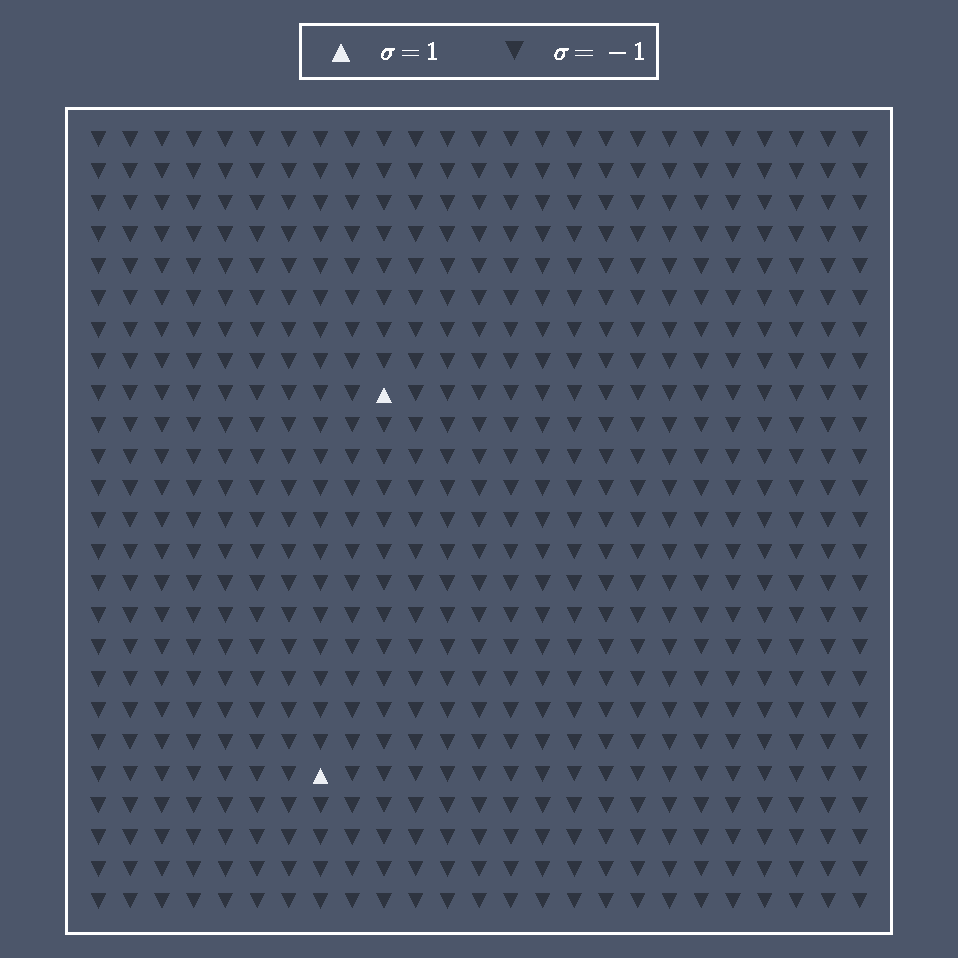
\includegraphics[width=\textwidth]{imgs/hw7/system_T1_3.pdf}
        \caption{~}\label{fig9:finalStates_a}
    \end{subfigure}
    \begin{subfigure}[c]{0.3\textwidth}
        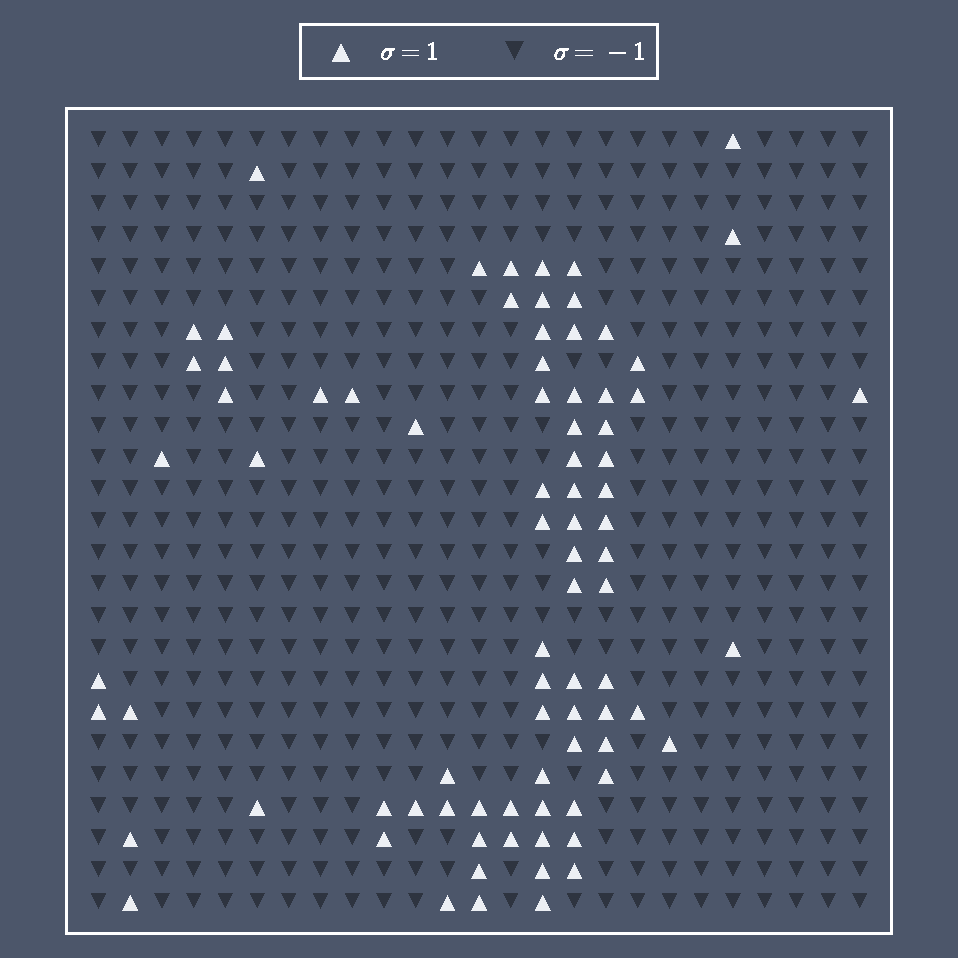
\includegraphics[width=\textwidth]{imgs/hw7/system_T2_3.pdf}
        \caption{~}\label{fig9:finalStates_b}
    \end{subfigure}\begin{subfigure}[c]{0.3\textwidth}
        
\includegraphics[width=\textwidth]{imgs/hw7/system_T3.pdf}
        \caption{~}\label{fig9:finalStates_c}
    \end{subfigure}
    
    \caption{Final configuration for cases with reduce temperature $T\in\{1.5,2.3,3\}$ from left to right.}
    \label{fig9:finalStates}
\end{figure}

On the other hand, in figure \ref{fig9:energyMagnetization}, is shown the energy and the magnetization of systems with temperatures of 1.3, 1.8, 2.4 and 3 for each Monte Carlo step.
In the energy plot, figure \ref{fig9:energyMagnetization_a}, the acceptance of states with higher energy can be easily seen in the system with lowest temperature, and, when increasing the temperature the algorithm start to allow a wider range of energetic states.
In the case of the magnetization, figure \ref{fig9:energyMagnetization_b}, the system tends to not have magnetization at higher temperatures, this is expected, because the amount of particles with opposite spin tends to increase.

\begin{figure}
    \centering
    \begin{subfigure}[c]{0.45\textwidth}
        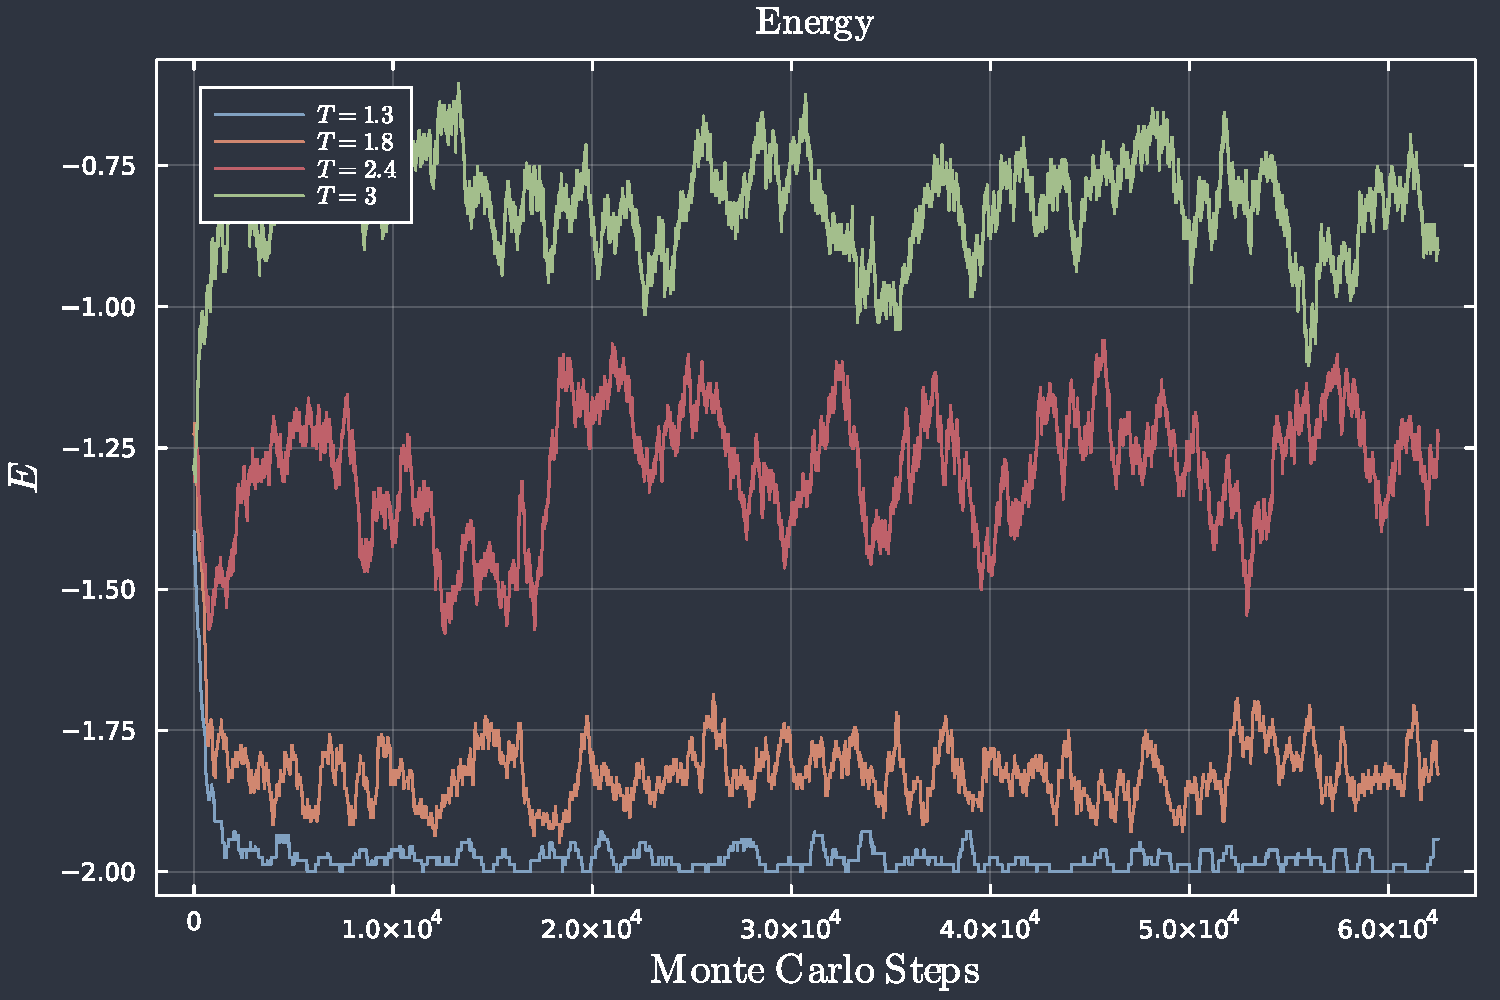
\includegraphics[width=\textwidth]{imgs/hw7/energyN25MOnteCarlosteps.pdf}
        \caption{~}\label{fig9:energyMagnetization_a}
    \end{subfigure}
    \begin{subfigure}[c]{0.45\textwidth}
        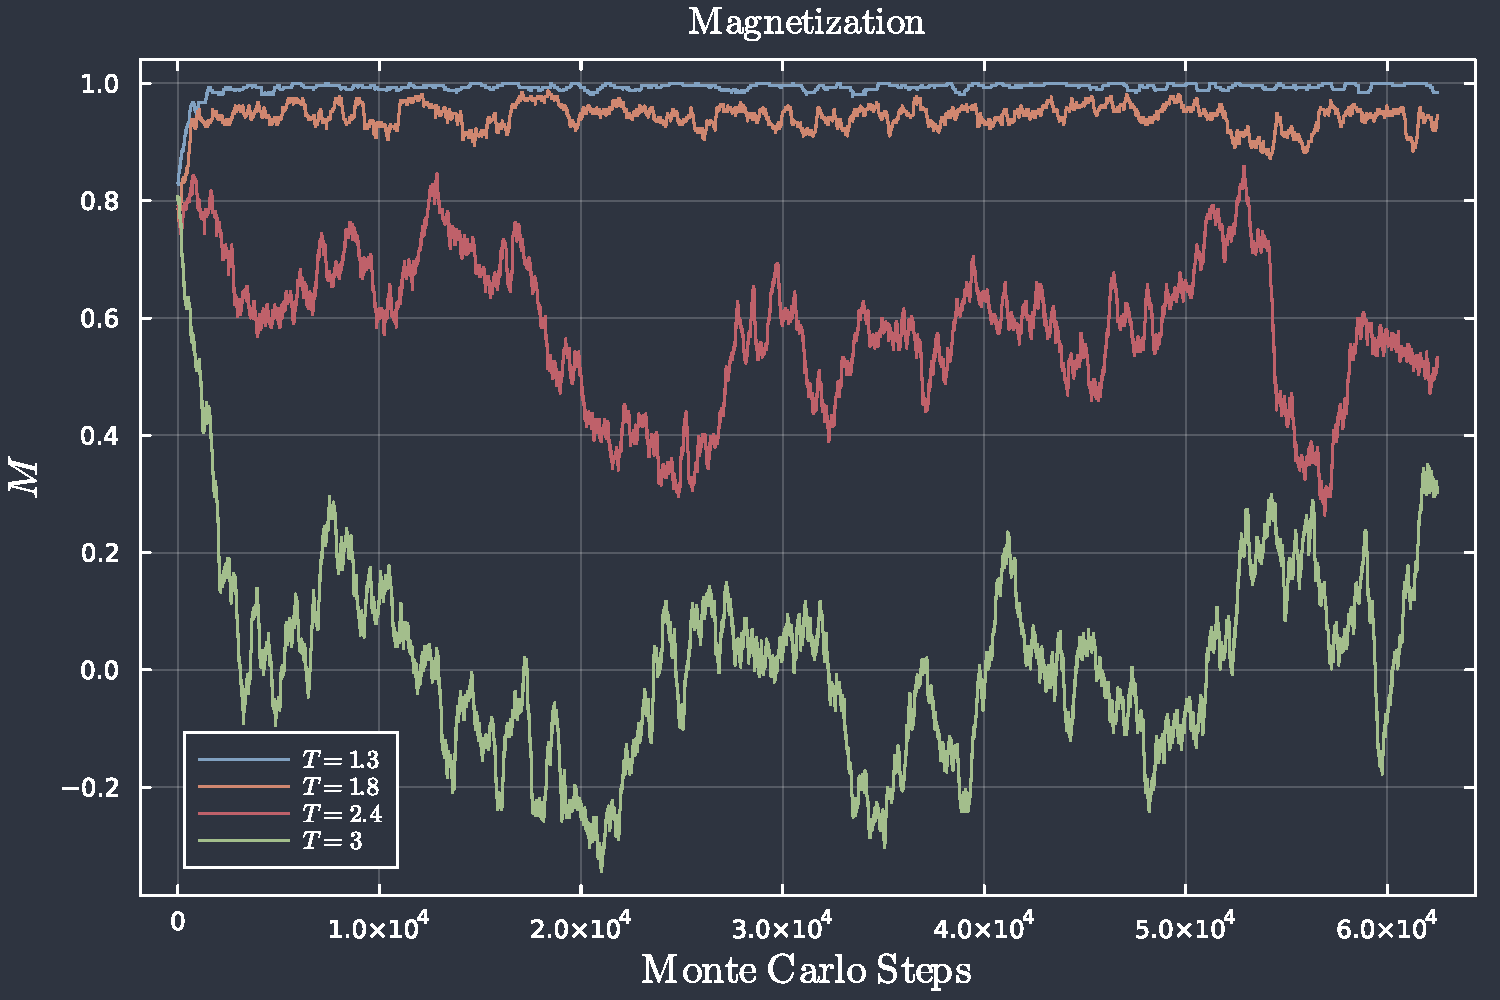
\includegraphics[width=\textwidth]{imgs/hw7/magnetizationN25MOnteCarlosteps.pdf}
        \caption{~}\label{fig9:energyMagnetization_b}
    \end{subfigure}
    \caption{Energy and Magnetization for $T\in\{1.3,1.8,2.4,3\}$}
    \label{fig9:energyMagnetization}
\end{figure}

Finally, in figure \ref{fig9:meanstd} is shown the average and variance of the energy and magnetization of 100 experiments in a temperature range, of 100 elements, from \num{1.3} to \num{3.0} and with three different system size, 5 by 5, 15 by 15 and 25 by 25 particles. 

The variance of the energy and the variance of the magnetization tends to "localize" around the temperatures of 2.2 and 2.4 when the number of particles in the system increases.
The average energy, figure \ref{fig9:meanstd_a}, tends to increase when the temperature increases and when the average of the systems of 15 by 15 and 25 by 25 are very similar, mean while, the system of 5 by 5 particles starts to differs with respect the other around a temperature of 2.
On the other hand, the average of the absolute value of the magnetization, figure \ref{fig9:meanstd_a}, tends to decrease at higher temperatures and the difference between the size of the system are more noticeable, finally, when the number of the particles in the system increases the average approaches zero.

\begin{figure}
    \centering
    \begin{subfigure}[c]{0.45\textwidth}
        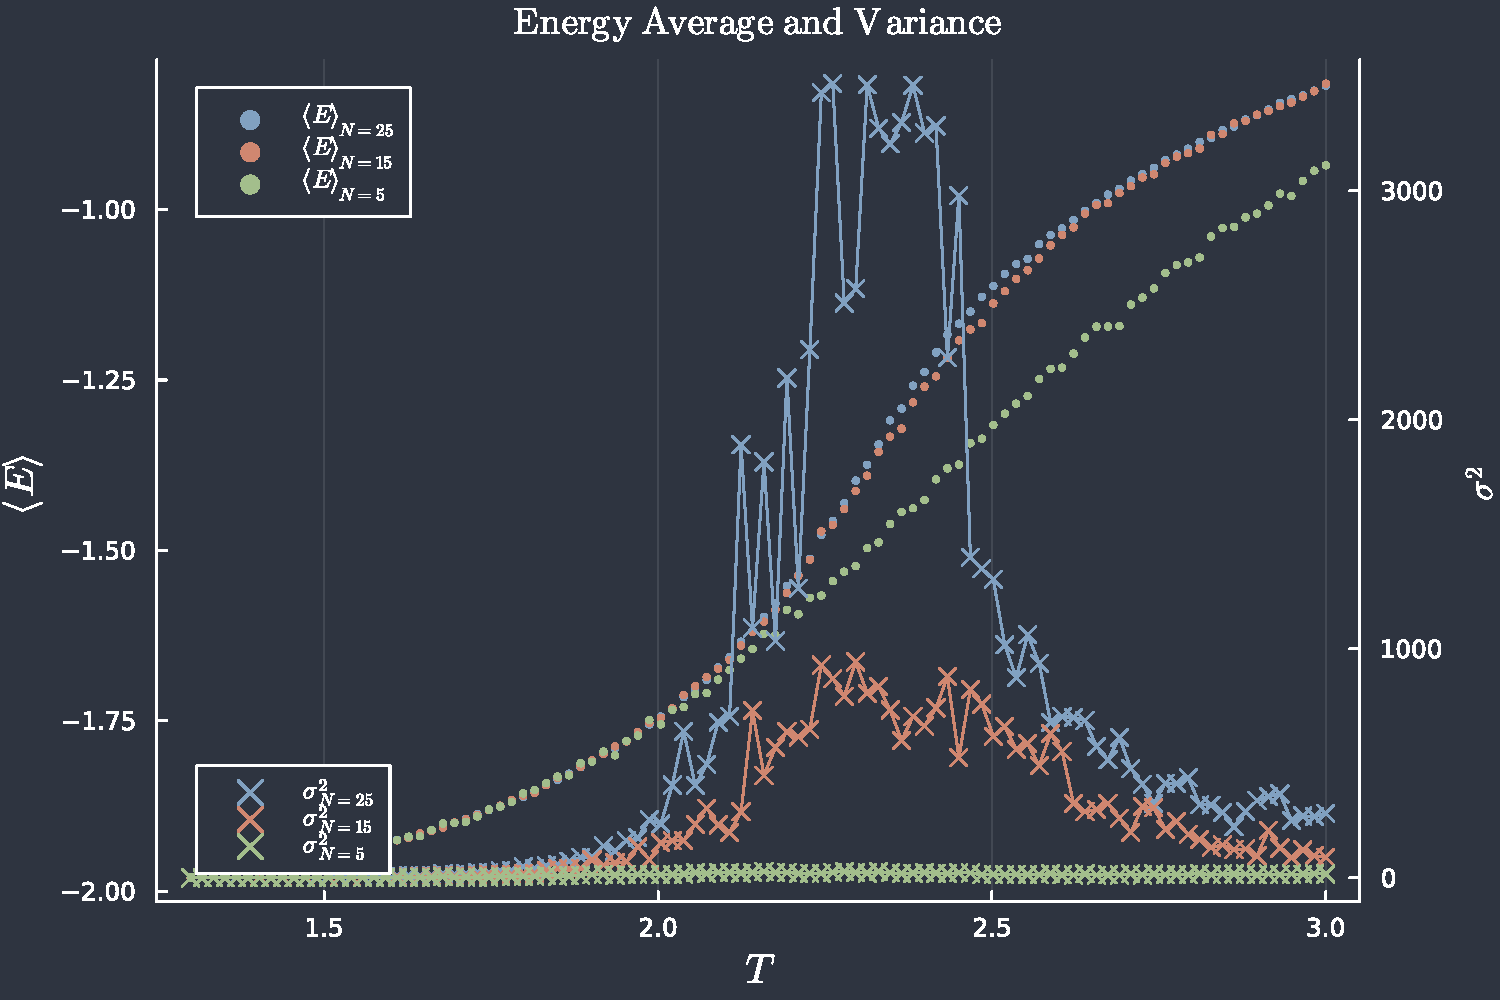
\includegraphics[width=\textwidth]{imgs/hw7/energyMean.pdf}
        \caption{~}\label{fig9:meanstd_a}
    \end{subfigure}
    \begin{subfigure}[c]{0.45\textwidth}
        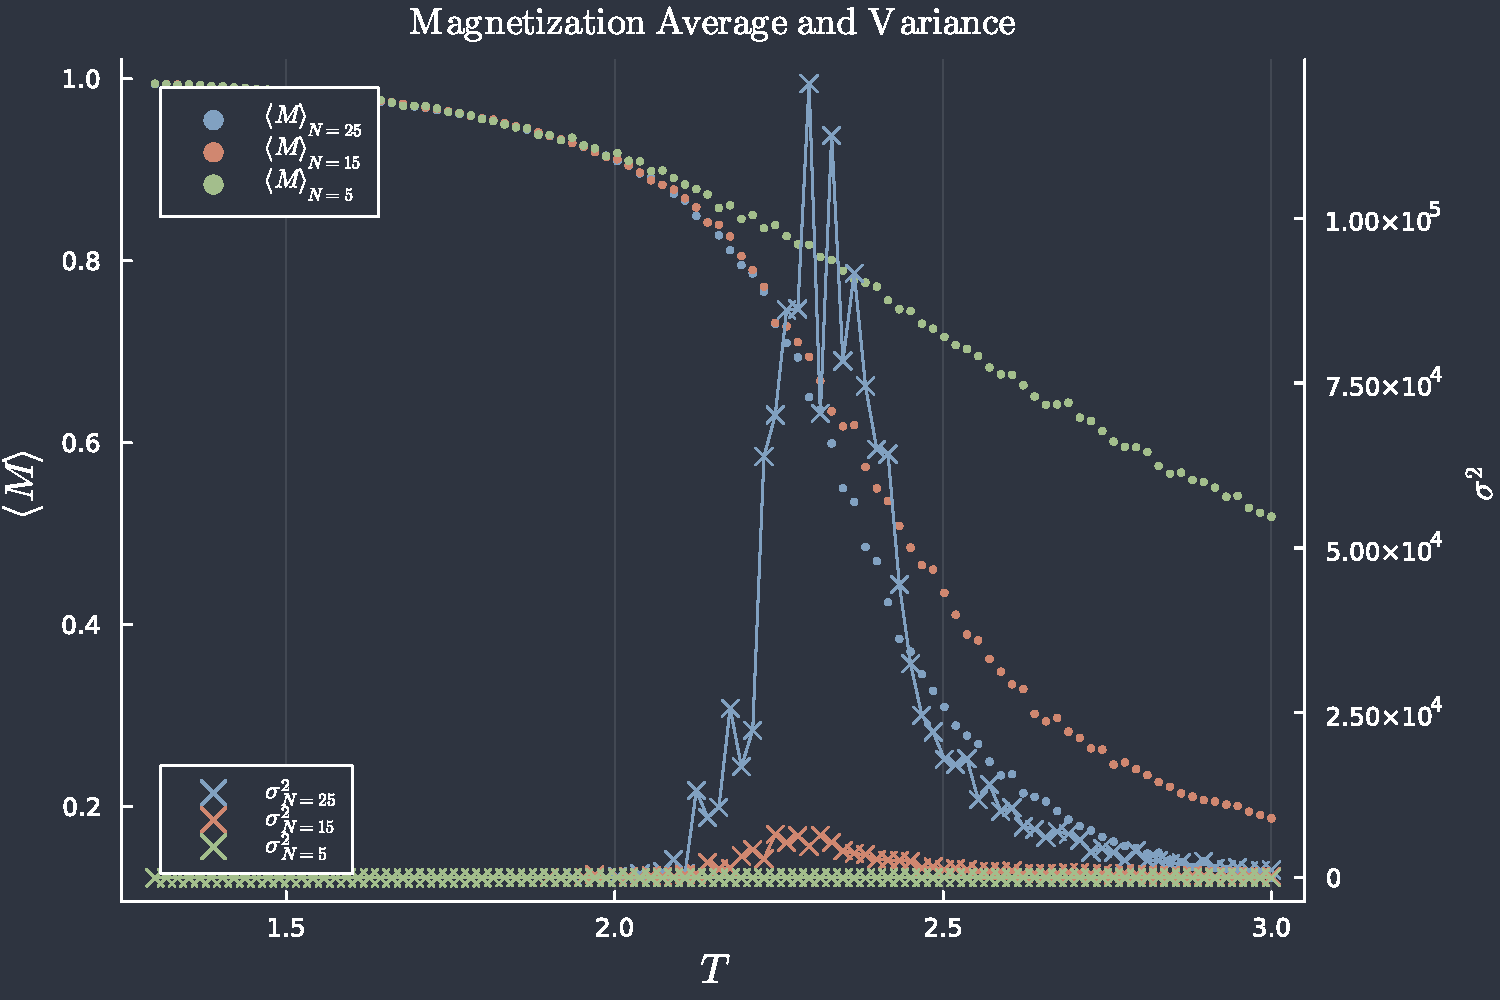
\includegraphics[width=\textwidth]{imgs/hw7/magnetizationMean.pdf}
        \caption{~}
    \end{subfigure}\label{fig9:meanstd_b}
    \caption{Average and variance of the energy and the absolute value of the magnetization for $T\in\{1.3,1.8,2.4,3\}$}
    \label{fig9:meanstd}
\end{figure}



% http://micro.stanford.edu/~caiwei/me334/Chap12_Ising_Model_v04.pdf



\end{document}